%
% File nlp-report-isabella.tex
%
% % Based on semeval 2020 Nathan Schneider
%% Based on the style files for COLING-2020 (feiliu@cs.ucf.edu & liang.huang.sh@gmail.com), which were, in turn,
%% Based on the style files for COLING-2018, which were, in turn,
%% Based on the style files for COLING-2016, which were, in turn,
%% Based on the style files for COLING-2014, which were, in turn,
%% Based on the style files for ACL-2014, which were, in turn,
%% Based on the style files for ACL-2013, which were, in turn,
%% Based on the style files for ACL-2012, which were, in turn,
%% based on the style files for ACL-2011, which were, in turn, 
%% based on the style files for ACL-2010, which were, in turn, 
%% based on the style files for ACL-IJCNLP-2009, which were, in turn,
%% based on the style files for EACL-2009 and IJCNLP-2008...

%% Based on the style files for EACL 2006 by 
%%e.agirre@ehu.es or Sergi.Balari@uab.es
%% and that of ACL 08 by Joakim Nivre and Noah Smith

\documentclass[11pt]{article}
\usepackage{geometry}
\usepackage{coling2020}
\usepackage{times}
\usepackage{url}
\usepackage{latexsym}
\usepackage{microtype}
\usepackage{listings}
\hyphenation{an-aly-sis}
\hyphenation{an-aly-ses}
\hyphenation{Sem-Eval}
\usepackage[dvipsnames]{xcolor}
\usepackage{hyperref}
\hypersetup{
    colorlinks=true,
    linkcolor=Emerald,
    filecolor=magenta,
    urlcolor=blue,
    citecolor=RoyalBlue
}
\usepackage{graphicx}
\graphicspath{ {./images/} }
\setlength\titlebox{5cm}
\colingfinalcopy

\title{SemEval-2020 Task 1: Dialogue and Narrative Coursework Report}
\author{Isabella Degen \\ University of Bristol \\ {\tt isabella.degen@bristol.ac.uk}}
\date{}

\begin{document}
    \maketitle

    \begin{abstract}
        How does an embeddings based approach for finding the grounding documents to a user question compare to ....

    \end{abstract}

    focus on developing your understanding of designing,  building,  and evaluating an NLP system.
    We are looking for a scientific approach to designing and evaluating the system and a technically sound implementation,
    based on what we have learned during the unit.


    \section{Introduction}\label{sec:introduction}
    Motivation and Approach:

    This report describes the method, experiment setup, results and conclusions for the 2021 Dialogue and Narrative
    coursework.

    The aim of this coursework was to gain more experience and to apply some of the NLP techniques we've learned during
    the semester. I focused on designing, implementing and evaluating a simple embeddings based solution for
    subtask 1 from the DialDoc21
    competition \cite{feng-etal-2020-doc2dial}.
    This allowed me to learn how a simple solution compares to the submissions that topped the leaderboard,
    while developing my python programing skills and
    learing how to implement, evaluate and keep track of experiments and results for an NLP system.

    I started with building my understanding about the Doc2Dial dataset \cite{feng-etal-2020-doc2dial} using Jupyter notebooks
    before experimenting with an embeddings algorithm called Doc2Vec from Gensim \cite{rehurek_lrec}.
    To run multiple experiments and vary with the hyperparameters of the system,
    I moved the Python code into a Python module, wrote Unit Tests for the important functions, moved the configuration
    into a Configuration Dataclass and logged each experiment using
    the Weights \& Biases platform \cite{wandb}. For the rest of this report I'm going to refer to the Weights \& Biases
    as wandb

    The following sections go into more details about each step.

%    TODO - how to be able to reproduce an experiment?
    Conda environment for this coursework build from the conda.yml file. Only version fixed is Python 3.9 as I want
    to use the latest versions for all other libraries. Wandb \cite{wandb} automatically produces an \texttt{requirements.txt}
    file for each run that lists the exact version of each library at the time of the run to help with reproducibility.


    \section{Technical Background}\label{sec:technical-background}

    - Describe Doc2Vec background
    - Describe Wand

    Include https://arxiv.org/abs/1405.4053v2


    \section{Method}\label{sec:method}

    \subsection{Understanding the Data}\label{subsec:understanding-the-data-method}
    Before starting to develop an algorithm I wanted to get an understanding of the dat available.
    There are three datasets for the Doc2dial competition available on \href{https://huggingface.co/datasets/doc2dial}{Hugging Face}:
    \begin{itemize}
        \item dialogue\_domain with data split train and validation
        \item document\_domain with data split train
        \item doc2dial\_rc with data split train and validation
    \end{itemize}

    I wanted to answer the following questions:
    \begin{itemize}
        \item What are the different datasets and how can I use them?
        \item How many grounding documents where there?
        \item How were they used in the dialogue?, How do I know which document was referenced in the dialogue?
        \item What was the format and type of the data?, What data type was the data?,
        Was the document already split into spans and how?
        \item How much data do I have?. How many spans does a document have?, How often is each span used in the dialogue?,
        Was each document used?
        \item How do I best interact and query the dataset?,Do I continue to use panda's dataframe or do I directly query
        the arrow dataset?
    \end{itemize}


    \subsection*{Random Guessing as Baseline}\label{subsec:random-guessing-method}

    Before diving into an NLP algorithm solution to subtask1, I wanted gain an idea of how well a program that randomly guessed a
    grounding span scores. This served me as baseline for the rest of the work.




    \section{Experiment Setup}\label{sec:experiment-setup}

    All experiments were run within the nlp-2021 conda environment on my mac. The conda environment is built and updated using the
    \href{https://github.com/isabelladegen/nlp-2021/blob/main/conda.yml}{conda.yml} file. The
    \href{https://github.com/isabelladegen/nlp-2021}{Readme} on Github describes how to setup the environment as well
    as how to run a wandb experiment.

    \subsection{Understanding the Data}\label{subsec:understanding-the-data-experiment}
    I analysed the three datasets dialogue\_domain, document\_domain and doc2dial\_rc using the Jupyter Notebooks
    \href{https://github.com/isabelladegen/nlp-2021/blob/main/notebooks/DataInvestigationDoc2Dial.ipynb}{DataInvestigationDoc2Dial.ipynb}
    and \href{https://github.com/isabelladegen/nlp-2021/blob/main/notebooks/RCDataInvestigation.ipynb}{RCDataInvestigation.ipynb}.
    The notebooks download the downloaded from \href{https://huggingface.co/datasets/doc2dial}{Hugging Face}
    using \texttt{load\_datasets} and import into pandas dataframes \cite{reback2020pandas} to make use of
    \texttt{describe()}, \texttt{info()}, \texttt{value\_counts()}, \texttt{json\_normalize()}. To gain more insights
    about how the grounding documents from \texttt{document\_domain} are used in in the \texttt{dialogue\_domain},
    I wrote a procedure to combine the two and and count for each document the number of dialogs, number of turns, number of user utterances,
    number of agent utterances, number of spans, number of references to the most used span, number of spans that are never referenced.
    I also wrote a procedure to combine the \texttt{doc2dial\_rc} with \texttt{dialogue\_domain} dataset so I could understand
    this data set better. I used \texttt{matplotlib} \cite{matplotlib} and \texttt{seaborn} \cite{seaborn} to visualise
    some of my findings.

    \subsection*{Random Guessing as Baseline}\label{subsec:random-guessing-experiment}
    For random guessing I loop through each of the questions in the \texttt{doc2dial\_rc} datataset and simply guess a
    random span id from the number of spans for the grounding document. The code for this can be found at the
    bottom of the 


    \section{Results}\label{sec:results}

    \subsection{Understanding the Data}\label{subsec:understanding-the-data-results}

    The \textbf{\texttt{dialogue\_domain}} dataset contains all the different dialogues. The grounding document is referenced
    by \texttt{doc\_id}, the dialogue history can be found in \texttt{turns} with \texttt{utterance} being the question
    or answer by either the user or the agent marked with \texttt{role}. In \texttt{turns.references.sp\_id} the list of
    matching span ids for the grounding document is provided.

    \begin{figure}[h]
        \centering
        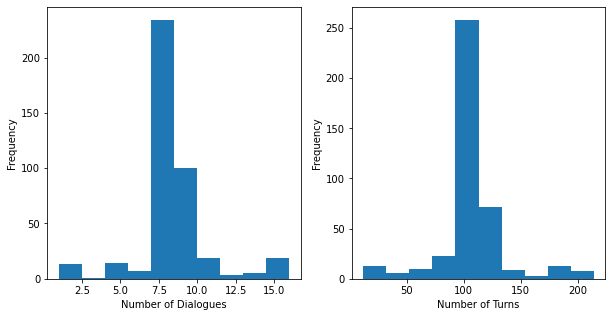
\includegraphics[width=0.8\textwidth]{number_of_dialogues_and_turns}
        \caption{Histograms for the number of dialogues per document and the number of turns per dialogue}
        \label{fig:histogram-dialogue-and-turns}
    \end{figure}

    In total there are 3474 different dialogues in the training dataset. For each document there are around eight dialogues and
    each dialogue has around a 100 turns, see figure \ref{fig:histogram-dialogue-and-turns} for teh histograms of the numbers of
    dialogues for each document and the number of turns in each dialogue.
    The training dialogue dataset only uses 415 of the 488 grounding documents.\\

    The \textbf{\texttt{document\_domain}} dataset contains all the different grounding documents. Note that this dataset does not have
    a training and validation data split and all documents used for training and validation are in the train split.
    The documents share the same \texttt{doc\_id} with the \texttt{dialogue\_domain}. The full text of the document
    can be found in \texttt{doc\_text}. The documents are already preprocessed into spans \texttt{spans} which themselves
    use the \texttt{id\_sp} that then refers back to the \texttt{sp\_id} used in the dialogue's turns. The \texttt{text\_sp}
    contains the span text.

    \begin{figure}[h]
        \centering
        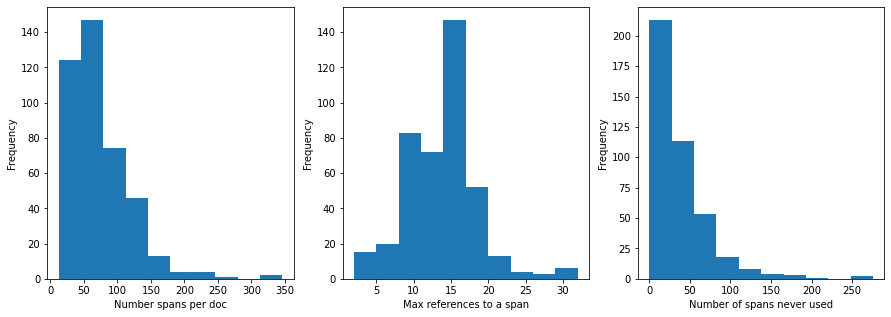
\includegraphics[width=0.8\textwidth]{span_counts}
        \caption{Histograms for the number of spans per document, the max number of references to the same span in a dialogue and the number of
        spans never referenced in a dialogue }
        \label{fig:histogram-spans}
    \end{figure}

    There are 488 different grounding documents in the dataset that come from 5 different domains. Each document has
    around 50 different spans. Some spans are referenced multiple times in a dialogue, the max number of references
    to the same span are around 16. Most documents have spans that are never used, this is usually in the tens but for a few documents
    this is significantly higher; see figure \ref{fig:histogram-spans} for the histograms.

    I also created a heat map to visualise how frequent the spans from the different documents were used in the \texttt{dialogue\_domain},
    see figure \ref{fig:heat-map-all-spans}. Given that the documents have different numbers of span, I set the frequency for spans that did not exist to -10. These
    are therefore shown as the darkest colour in the figure. Bighter colours mean that spans is referenced more frequently in a
    dialogue. I also included a figure that shows the heatmap just for the first 30 documents and their first 30 spans
    so the numbers become visible, see figure \ref{fig:heat-map-first-30-spans}. Both graphics show that most spans
    are hardly ever referenced and a few are very frequently referenced. This needs to be taken into account when
    deciding which algorithm is going to be used used to learn what's the best grounding span for a user utterance.

    \begin{figure}[h]
        \centering
        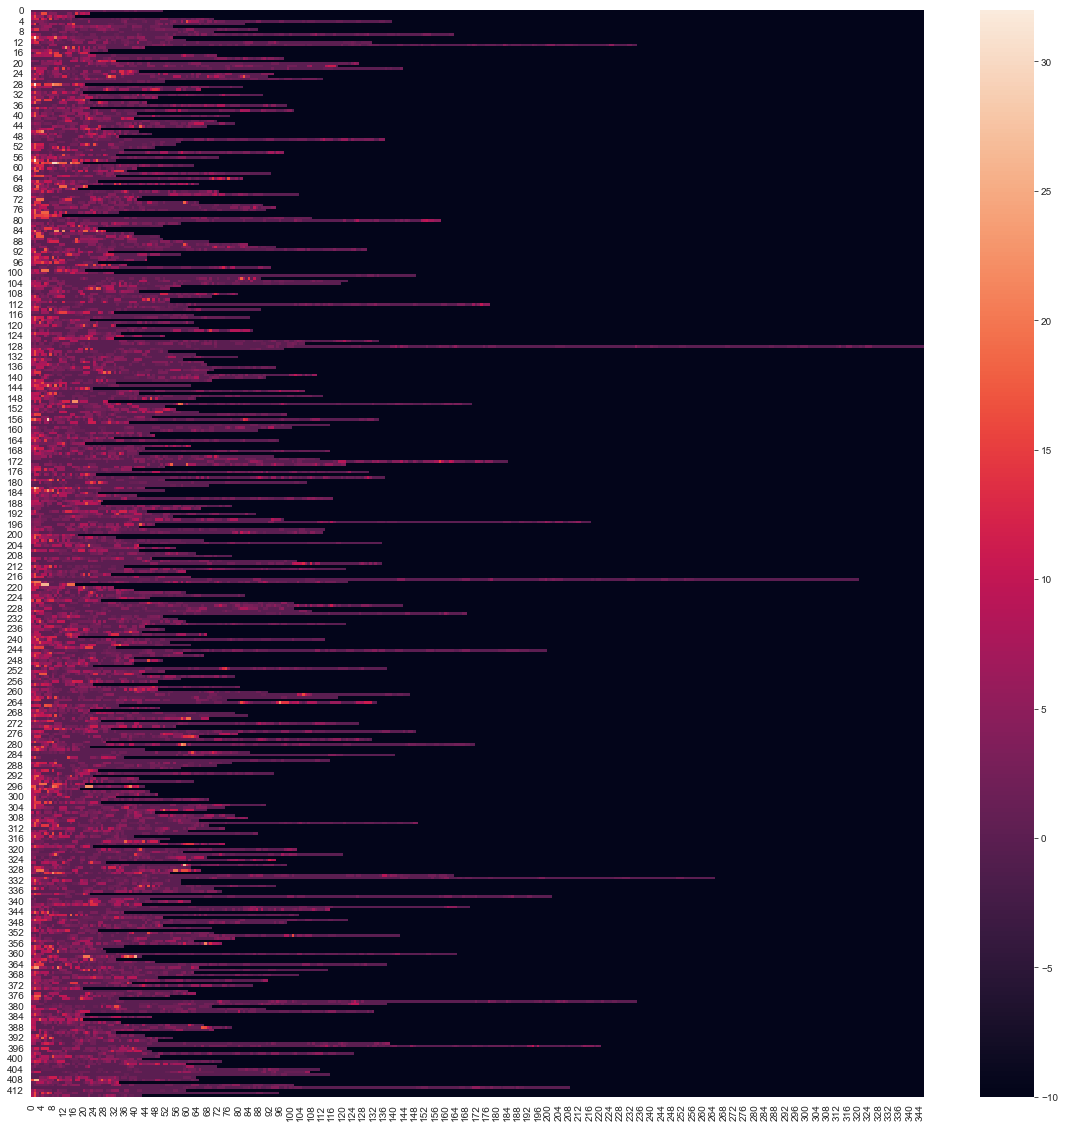
\includegraphics[width=0.8\textwidth]{sparsity_of_spans}
        \caption{Heat map of the frequency a span is referenced in a dialogue. Bright fields indicate spans that are frequently
        referenced in a dialogue, black means that span does not exist in that document}
        \label{fig:heat-map-all-spans}
    \end{figure}

    \begin{figure}[h]
        \centering
        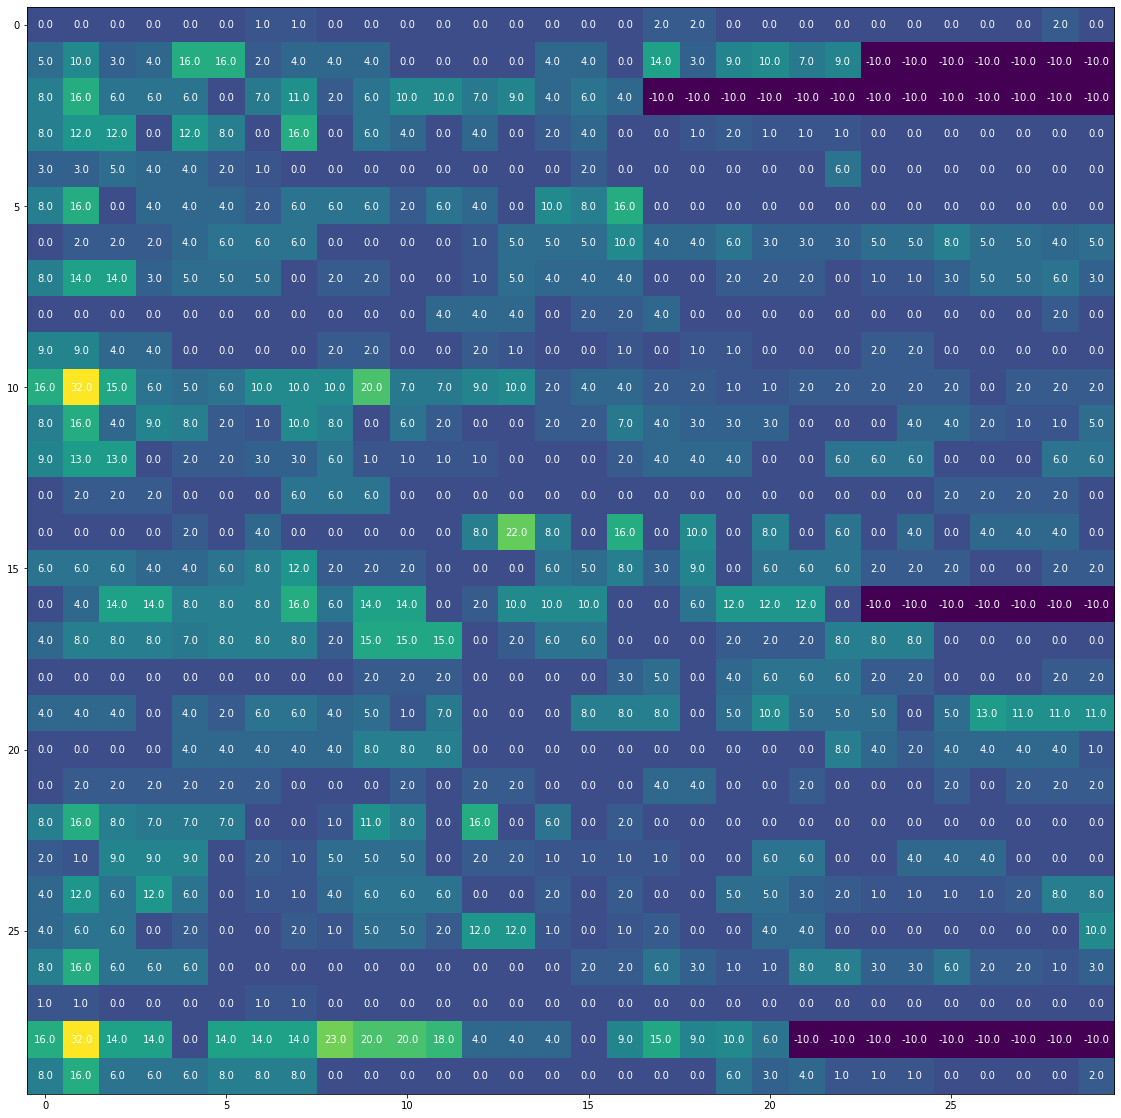
\includegraphics[width=0.8\textwidth]{sub_section_usage_of_spans}
        \caption{Heat map of the first 30 documents and the number of references to their first 30 spans. Violet or the number
        -10 indicates the span did not exist}
        \label{fig:heat-map-first-30-spans}
    \end{figure}

    Initially, I thought I needed to create a list of user utterances and the dialogue history for which I need to find the
    grounding document myself using the \texttt{turns} from the \texttt{dialogue\_domain} dataset. When investigating how
    to get the already provided \href{https://github.com/doc2dial/sharedtask-dialdoc2021/blob/master/scripts/sharedtask_utils.py}{scoring script}
    to work did I learn that it was easiest to run my alogrithm of the \texttt{doc2dial\_rc} dataset already had this work done for me.
    This dataset refers to the grounding documents \texttt{doc\_id} by \texttt{title}.
    The \texttt{id} is the combination of the \texttt{dialogue\_id\_turn\_id}. \texttt{question} is the dialogue history starting
    with the the user question that the grounding document should be found for and listing the previous dialogue at each step.
    Utterances for the user are marked with a \texttt{user:}, those of the agent are marked with \texttt{agent:}. Not
    all user utterances have their own \texttt{doc2dial\_rc} data row. User's comments or confirmations, e.g \textit{Yes.} and
    \textit{Ok.} are omitted.



    Notes: about F1 scores and so the rest of the metrics is not in use if the no answer probability is not used (which was not part of the exercise
    see \cite{squad2git}


    \section{Conclusions}\label{sec:conclusions}
    share any insights you gained about how the system works.
    - solution is inferior to any solution on the leaderboard but better than random guessing
    - F1 and exact match are hard to both optimise, better F1 means bad exact match
    -   problem came from me allowing the algorithm to return multiple spans that could be from all over the document.
    had I only allowed spans from the same sections with the highest probability F1 and exact match might not have been opposite

    - curious to know how well word2vec would have worked

    \subsection{Learnings}\label{subsec:learnings}
    - focus on building the end to end pipeline before diving into the data, endless time can be spent analysing the data
    but having an end to end process going actually helps focusing what areas need more analysis
    - keeping the data mangling code out of notebooks and in tested python code
    - Build configuration and experiment tracking in from the start, I lost a lot of time forgetting what I've tried before I
    moved to tracking all parameters on Weights and Biases


    \bibliographystyle{coling}
    \bibliography{bibliography}

\end{document}
